%======================================================================
%  Chapter : ベクトル解析
%  説明    : 電磁気学を記述する上で必要なベクトル解析のまとめ
%======================================================================

%======================================================================
%  Section
%======================================================================
    \section{ベクトル}
        \begin{mycomment}
        ここで述べるベクトル定義は,非数学的である.
        使うことが目的であり,ベクトル論の理論構築には興味がないので,
        直感的な定義で十分である.
        \end{mycomment}

                \subsection{ベクトルの定義}
        数字がいくつか並んだものを,1組の集まりとして認識し扱うとき,この
        1組の数の集まりを \textbf{ベクトル} という.
        数の集まりを $(a,\,b,\,c,\,\cdots)$のように表す.
        ベクトルとは,この数の集まりを1つの対象としてみるものである.

        このノートでは,ベクトルをアルファベットの太字で表す.例えば,
        \begin{align}
            \br := (a,\,b,\,c,\,\cdots)
        \end{align}
        と書く.

        他にも流儀があり,例えば,$\vec{a}$ のように上に矢印を書いたりすることも多い.
        また,ギリシャ文字($\alpha,\,\beta,\,\gamma,\,\cdots$)をベクトル,
        アルファベット($a,\,b,\,c,\,\cdots$)をスカラーと,書き分ける方法もある.

        \begin{memo}{ベクトルが使われる場面}
        位置の特定には,縦と横と高さの3つの数字を同時に指定する必要がある.
        例えば,$xyz$ 直交座標であれば,縦と横と高さを示す3つの数字が必要である.
        1次元であれば数字1つで良いのだが,3次元となると
        1つの数字では位置を一意に特定することはできない.
        3次元の位置情報を示すためには,3つの数字を同時に扱う必要があり,
        ベクトルという概念が使われる
            \footnote{
                数値計算で位置情報を扱うには,四元数と言われるベクトルと等価な概念
                を使うこともあるらしい.ベクトルだけが唯一の方法ではないということだ.
                計算機を使った数値的解法には四元数が向いていて,
                手計算による解析的解法では,ベクトル解析が重宝される.
            }.
        \end{memo}

        \subsection{成分}
        \begin{mysmallsec}{成分の意味}
        ベクトルを $\br = (x,\,y,\,z)$ のような
        記述方法を \textbf{成分表示} という.
        また,この $x$,$y$,$z$ を
        ベクトル $\br$ の \textbf{成分} という.
        \end{mysmallsec}

        \begin{mysmallsec}{添字記号の導入}
        次元数が多い場合,$x$,$y$,$z$ のように異なる文字を使っていると,
        使用できる文字が尽きてしまう.アルファベットだけでは最大で26次元までしか
        表現できない
            \footnote{
                アルファベットの種類数は26である.
            }.
        新しい文字を作るという策もあるが,もっと効率の良い方法がある.
        その方法とは,成分の文字を細字にして,添字に数字を使用することである.
        そうすると,例えば,
            \begin{equation*}
                \ba = (a_{1},\,a_{2},\,\cdots,\,a_{100},\,a_{101},\,\cdots)
            \end{equation*}
        のように書ける.こうすれば,新しい文字を作ることなしに,
        いくらでも次元数を大きくできる
            \footnote{
                "原理的には" という但し書きが付くけれど$\cdots$.
                次元数があまりにも大きいと,添字の数字を書くのに手間なのだ.
                100とか1000とかだったらよいが,1兆とか1京とかとなると,
                お手上げだ.指数を使うと良いのかもしれないが$\cdots$.
                ここではこれ以上の表記方法へのツッコミはしないでおく.
            }.

        任意の成分を表したい場合は,添字記号 $i$ を導入して,$a_{i}$ と書く.
        $i$ は1から$n$ までの自然数の内の,どれか1つである.

        いくつかの成分をまとめて表したい場合は,
        添字記号を活用し,以下のように表すこともできる.
        例えば,偶数番目の成分を表現したければ,
            \begin{equation*}
                a_{i} \quad,\quad (i\mbox{は偶数})
            \end{equation*}
        のように記述すれば良い.
        これは,$a_{2},\,a_{4},\,\cdots$ の別表現であり,同じことを言っている.
        成分の横に,条件を括弧で囲んでおけばいい.
        この表現の仕方で,すべての成分を表すと,
            \begin{equation*}
                a_{i} \quad,\quad (i=1,\,2,\,3,\,\cdots)
            \end{equation*}
        となる.この条件式には,集合論で使われる記号が用いられることも多い.

        添字 $i$ の範囲が一度示されたあとは,単に $a_{i}$ と記述されるので,
        $i$ の条件は常に意識しておくべきだ.
        \end{mysmallsec}

        \subsection{対応する成分}
        2つのベクトルの添字の数字が等しい成分同士を,\textbf{対応する成分} という.
        例えば,$\ba$ と $\bb$ の

        成分が ($a_{1},\,a_{2},\,\cdots$),($b_{1},\,b_{2},\,\cdots$) の場合の
        対応する成分とは,$a_{1}$ と $b_{1}$,$a_{2}$ と $b_{2}$,$\cdots$,の組をいう.

        \subsection{次元}
        ベクトルの成分の個数が有限である場合,これを \textbf{次元} という.
        成分の個数が $n$ 個ベクトルのことを  \textbf{$n$ 次元ベクトル} とよぶ.

        ベクトルの次元は,自然数である.
        今まで扱ってきた普通の数は,1次元ベクトルとみなすことができる.
        2次元以上のベクトルを総称して \textbf{多次元ベクトル} という.

        空間のみを考える場合は3次元ベクトルを使う.
        空間に加えて,時間を含めた場合は4次元ベクトルを扱う.
        現象が平面上で収まる場合には,2次元ベクトルを導入すればいい.

        \subsection{スカラー}
        ベクトルとの区別を強調するために,今まで扱ってきた普通の数のことを,
        \textbf{スカラー} ということがある.
        スカラーも1次元のベクトルであるが,区別したい場合がある.

        \subsection{定ベクトル}
        成分が全て定数であるベクトルを \textbf{定ベクトル},
        あるいは \textbf{定数ベクトル}という.

        \subsection{同値}
        2つの $n$ 次元のベクトル $\ba$,$\bb$ が \textbf{同値} であるとは,
        $\ba$ と $\bb$ の対応する成分同士がすべて等しい場合をいい,この場合に限る.
        $\ba$ と $\bb$ が同値であることを表すには,$\ba=\bb$ と書く.

        ベクトルの同値を数式で定義すると,次の通り.
        \begin{align}
            \ba=\bb
            \quad\Leftrightarrow\quad
            a_{i}=b_{i}\quad,\quad(i=1,\,2,\,\cdots,\,n).
        \end{align}

        \subsection{ゼロベクトル$\bzero$}
        成分がすべて0のベクトルを \textbf{ゼロベクトル} といい,$\bzero$ で表す.
        \begin{align}
            \bzero := (0,\,0,\,\cdots,\,0).
        \end{align}

        \subsection{大きさ}
        $n$ 次元ベクトル $\ba$ の \textbf{大きさ} を $|\ba|$ と表し,以下で定義する.
        \begin{align}
            |\ba| &:= \sqrt{\sum_{i=1}^{n} {a_{i}}^{2}}  \\ \notag \\
                  &=  \sqrt{{a_{1}}^{2} + {a_{2}}^{2} + \cdots + {a_{n}}^{2}}. \notag
        \end{align}

        具体的な例を示したほうが理解が早い.例えば,$n=2$ のときは,
        \begin{equation*}
            |\ba| = \sqrt{{{a}_{1}}^{2}+{{a}_{2}}^{2}}.
        \end{equation*}
        図形的なイメージは次の通り.三平方の定理が応用されていることが見えてくるはず.
        \begin{figure}[htbp]
            \begin{center}
                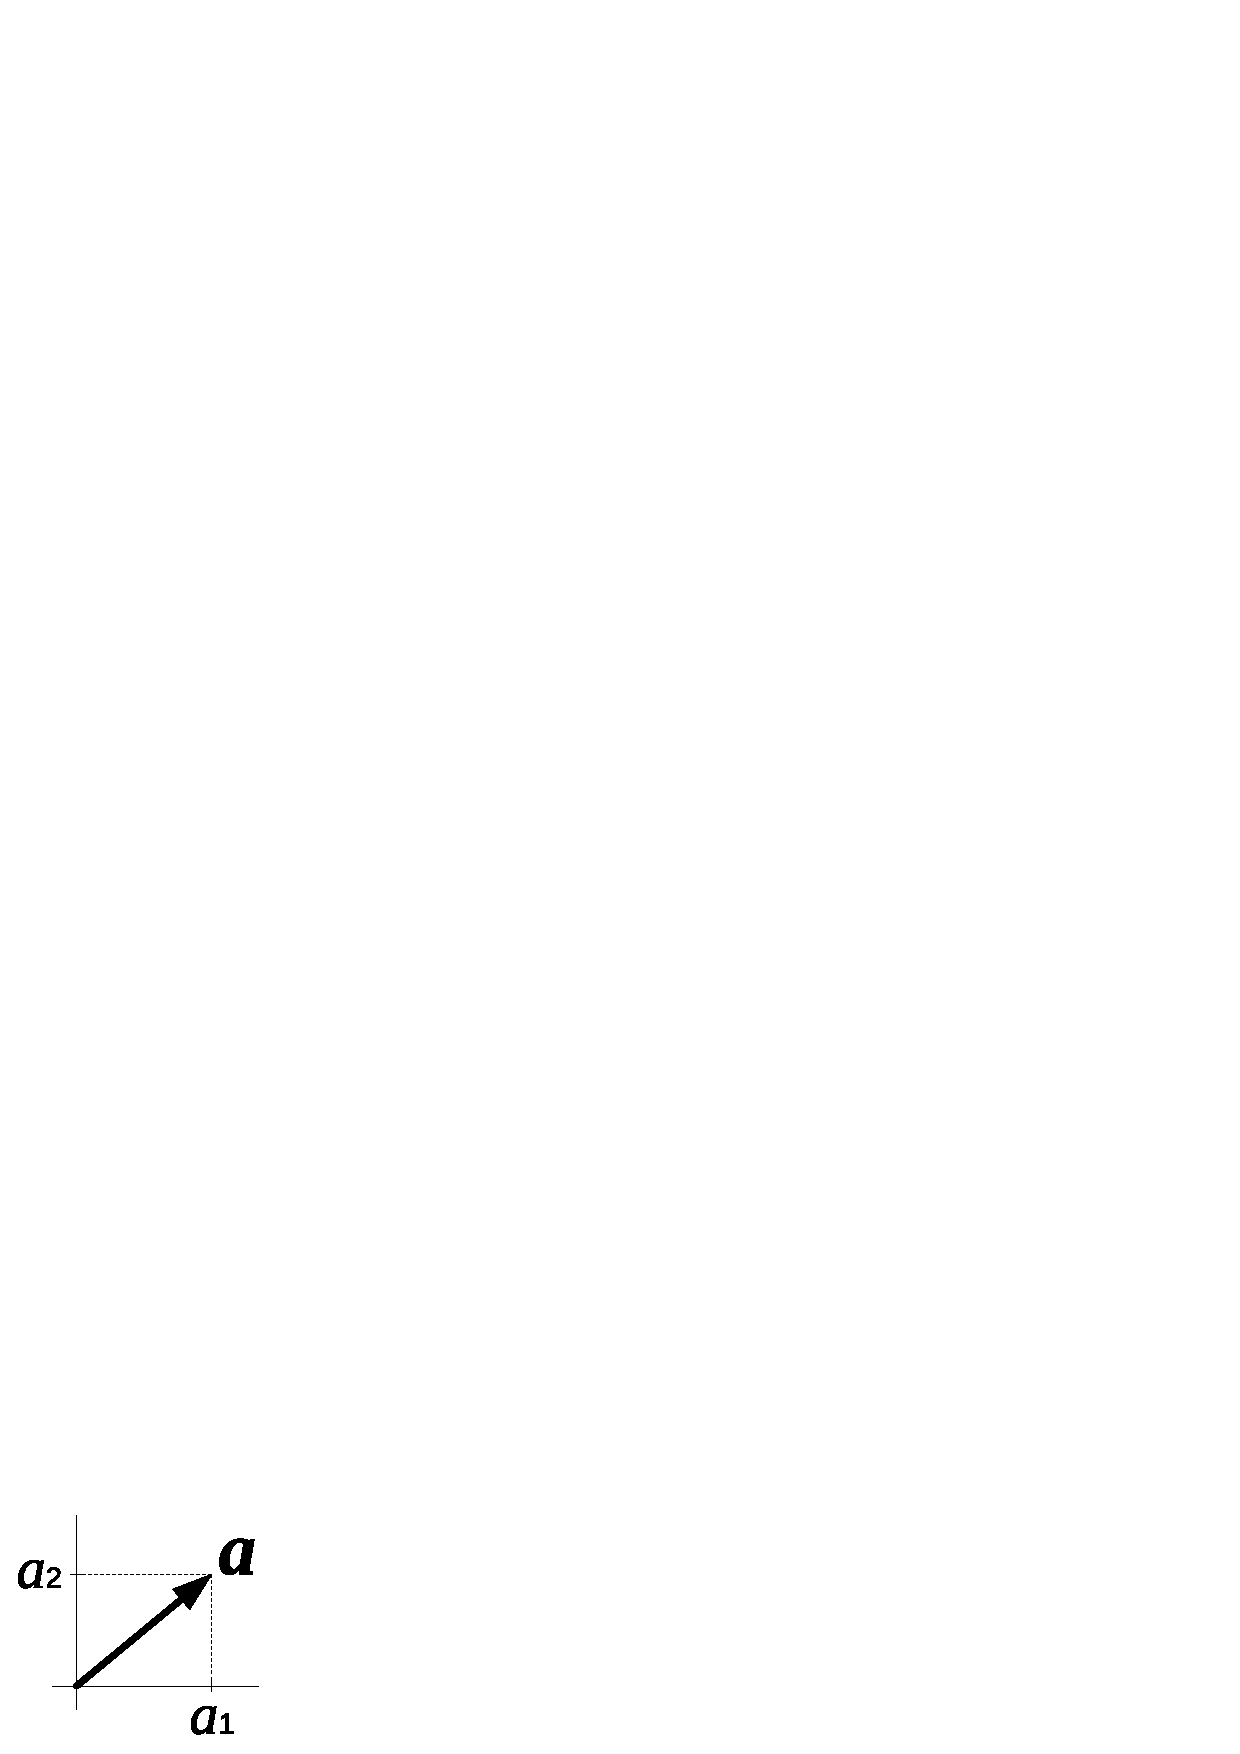
\includegraphics[keepaspectratio, width=3.1cm,height=3cm,clip]{chap9_ookisa001.pdf}
                \caption{2次元ベクトルの大きさ}
                \label{fig:chap9_ookisa001}
            \end{center}
        \end{figure}

        \subsection{基本演算}
        複数のベクトルがあるとき,ベクトル同士の演算を定義しておこう.
        ベクトルに対して定義される演算は,加算と減算と乗算であり,
        除算は定義されない.乗算には,
        定数倍,内積(スカラー積),外積(ベクトル積)の3種類がある.
        しかし,ここで言うベクトルの乗算は,
        普通の数で行われる乗算とは異なる概念であることに注意されたい
            \footnote{
                違いは,この後の説明で,自ずとわかるはず.
            }.
        ベクトルの演算が定義できるのは,すべてのベクトルの次元が同じ場合に限る.
        以下のベクトル演算の定義にでてくるベクトルは,すべて $n$ 次元
        ベクトルであると仮定する.次元が異なるベクトル同士の演算は定義しない.

        数学的な演算公理を示すことはせず,直感的にわかりやすい表現で
        演算の定義を示すにとどめておこう.

        \subsubsection{加算}
        2つの $n$ 次元ベクトル $\ba$,$\bb$ があるとき,
        この2つのベクトルに対する演算 $\ba+\bb$ を \textbf{加算} といい,
        次のように定義する.
        \begin{align}
            \ba + \bb   &:= (a_{1},\, a_{2},\,\cdots,\,a_{n}) + (b_{1},\,b_{2},\,\cdots,\, b_{n}) \notag \\
                        &=  (a_{1}+b_{1},\, a_{2}+b_{2},\,\cdots,\, a_{n}+b_{n} ).
        \end{align}

        成分を示す場合には,次のようになる.
        \begin{align}
            {(\ba+\bb)}_{i} := a_{i}+b_{i} \quad,\quad (i=1,\,2,\,\cdots,\,n).
        \end{align}
        添字の $i$ はベクトルの成分番号を示している記号である.式はすべての成分で
        成り立つが,すべての成分を書くと,上の定義のように,$i=1,\,2,\,\cdots,\,n$ の $n$ 通り
        を記述する必要が出てくる.しかし,どの成分番号に対しても,同じ形の式で
        定義で定義されることから,1から$n$の任意の一つを代表的に表す $i$ を導入した.

        \subsubsection{定数倍}
        スカラー $k$ と $n$ 次元ベクトル $\ba$ の積 $k\ba$ を \textbf{定数倍} といい,
        次で定義する.ここでは,$k$ を実数とする.
        \begin{align}
            k\ba := (k{a}_{1},\, k{a}_{2},\, \cdots,\, k{a}_{n}).
        \end{align}
        $\ba$ のすべての成分を $k$ 倍するということである.

        成分を示す場合には,次のように書く.
        \begin{align}
            {(k\ba)}_{i} := k{a}_{i} \quad,\quad  (i=1,\,2,\,\cdots,\,n).
        \end{align}

        \subsubsection{減算}
        加算と定数倍を定義しておけば,減算を定義する必要はない
            \footnote{
                一方に$-1$を乗じて(乗算)から,たし合わせればいい(加算).
            }.
        しかし,特徴的な演算であるため,この演算に \textbf{減算} という呼称を与える.
        減算は以下のような演算でのことをいう.2つの $n$ 次元ベクトル $\ba$,$\bb$ があるとき,
        ベクトルの減算 $\ba-\bb$ とは,
        \begin{align*}
            \ba-\bb &:= \ba + (-1)\bb \\
                    &= (a_{1}+(-1)b_{1},\, a_{2}+(-1)b_{2},\,\cdots,\, a_{n}+(-1)b_{n} ) \\
                    &= (a_{1}-b_{1},\, a_{2}-b_{2},\,\cdots,\, a_{n}-b_{n} )
        \end{align*}
        のような演算のことである.

        成分を示す場合には,次のようになる.
        \begin{align}
            {(\ba-\bb)}_{i} := a_{i}-b_{i} \quad,\quad (i=1,\,2,\,\cdots,\,n).
        \end{align}

        \subsubsection{内積(スカラー積)}
        2つの$n$次元ベクトル $\ba$,$\bb$ の内積 $\ba\cdot\bb$ とは,以下の演算のことをいう.
        \begin{align}\label{eq:chap9_naiseki001}
            \ba\cdot\bb := \sum_{i=1}^{n} a_{i}b_{i}.
        \end{align}

        展開したほうが,見やすいかもしれない(同じことを書いているだけ).
        \begin{align}
            \ba\cdot\bb := a_{1}b_{1} + a_{2}b_{2} + \cdots + a_{n}b_{n}.
        \end{align}

        演算結果がスカラーになることから,\textbf{スカラー積} ということもある.

        2次元ベクトルの場合,内積には図形的なイメージがある.
        それを強調した場合の,内積の定義は以下の通り.
        \begin{align}
            \ba\cdot\bb := |\ba||\bb| \cos \theta.
        \end{align}
        この定義は上の式(\ref{eq:chap9_naiseki001})の $n=2$ の場合と同値である.
        証明は後回し.
        \begin{figure}[htbp]
            \begin{center}
                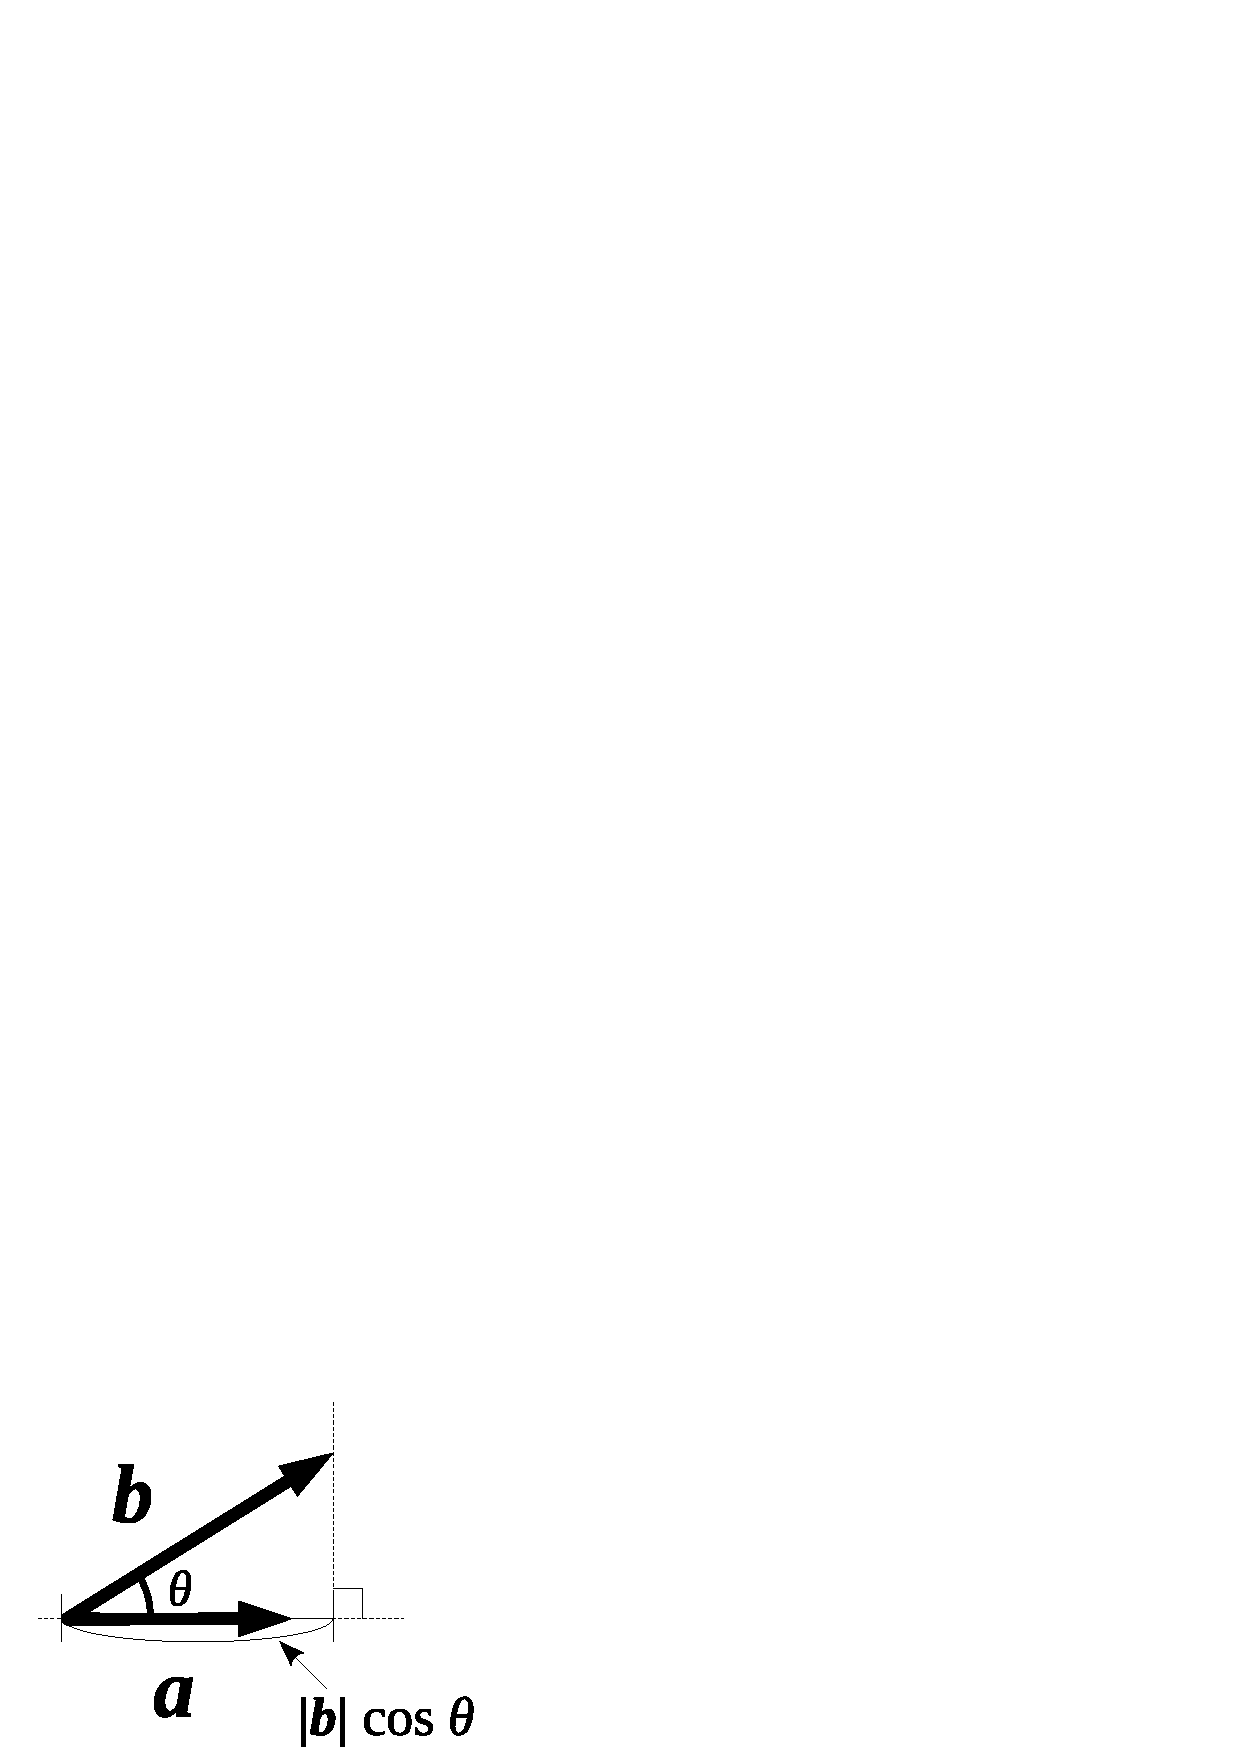
\includegraphics[keepaspectratio, width=4.23cm,height=3cm,clip]{chap9_naiseki001.pdf}
                \caption{内積}
                \label{fig:chap9_naiseki001}
            \end{center}
        \end{figure}

        \subsubsection{外積(ベクトル積)}
            \begin{mysmallsec}{外積の定義}
                2つの3次元ベクトル $\ba$,$\bb$ からなるベクトルの \textbf{外積} を
                $\ba\times\bb$ と表し,以下でその演算を定義する.
                    \begin{align*}
                            \ba \times \bb &:=& (\,
                                    a_{2}b_{3} - a_{3}b_{2},\;
                                    a_{3}b_{1} - a_{1}b_{3},\;
                                    a_{1}b_{2} - a_{2}b_{1}
                                \,)
                    \end{align*}

                演算結果がベクトルであることから,\textbf{ベクトル積} ということもある.

                唐突な定義で,無味乾燥だと思われるかもしれないが,
                根拠のあるものである.それを以下で説明しよう.
            \end{mysmallsec}

            \begin{mysmallsec}{一言}
                ベクトルの外積はわかりにくい.実際,定義式が少々複雑であり,図形的な
                イメージをすぐに描くには難しいかもしれない.しかし,ここを少々辛抱して
                手計算による練習をいくらかすることで,ベクトルの外積の意味やイメージを
                つかめるようになるはずである.
                ここでは,ベクトルの外積の定義を示すと共に,イメージを少しでも早くつかむ
                ことができるよう,丁寧に説明していく
            \end{mysmallsec}

            \begin{mysmallsec}{3次元ベクトルの外積のみを扱う}
                ここでの興味は3次元ベクトルの外積である.他の次元の外積は考えない.
                "興味がない"というのが直接的な理由だけれど,
                外積は内積のように簡単に $n$ 次元に拡張することができないことも,
                知っておいて損はないかも(多次元に拡張しようとして無駄な時間を費やさないように).

                外積の拡張に興味があれば,\textbf{外積代数} を学んでみる良い.
                外積代数は,ここでいう外積の自然な拡張ではないが(定義から違う),
                外積計算を発展させた形式の数学であることは実感できるだろう.
            \end{mysmallsec}

            \begin{mysmallsec}{定義の意味すること}
                ベクトルの外積とは,与えられた2つのベクトルから,
                この2つのベクトルの方向から独立した
                新しい方向を持つベクトルを1つ生成する演算である.
                その新しいベクトルの方向とは,2つのベクトルの両方に直交する方向であり,
                その大きさは $|\ba||\bb|\sin \theta$ である.
            \end{mysmallsec}

            \begin{mysmallsec}{外積の定義を知識0から作ろう}
                外積の定義の意味を実感するには,回り道かもしれないが,
                外積の定義に至るまでの思考プロセスをたどるとよい.
                先に示した外積の定義を一度忘れて,外積を1から作っていこう.
            \end{mysmallsec}

            \begin{mysmallsec}{外積の定義の目的}
                なぜ外積を定義したいのか.その理由は,外積を定義することにより,
                ある物理現象の数学的扱いが可能になるからである.必要は発明の母.
                力の釣り合いの解析には外積が欠かせないし,電磁気学ではローレンツ力
                を表すのに使われる.外積は闇雲に定義された演算ではなく,自然現象を
                詳細に観測した結果,それを説明するのに必要な演算方法なのである.
                自然現象の一部にはある特別な規則があり,それを数式で表そうとして
                試行錯誤して組み立てられた数学的概念が,外積なのである.
            \end{mysmallsec}

            \begin{mysmallsec}{外積演算に要求されること}
                2つの3次元ベクトル $\ba$,$\bb$ から,外積
                    \footnote{
                        今は,演算の名前なんてどうでも良い.知りたいのは
                        その具体的な演算方法である.この演算名は便宜的に
                        使用するものであり,"新しい演算方法"という
                        意味程度で捉えてもらいたい.
                    }
                によって生成したいベクトルの条件は以下の通りだった.
                \begin{enumerate}
                    \item 方向は $\ba$ と $\bb$ の両方に直交する方向である
                    \item 大きさは,$|\ba||\bb| \sin \theta$
                \end{enumerate}

                つまり,これから考えることは,
                \begin{enumerate}
                    \item 方向は 2つのベクトルに直交するようなベクトルをどう作るか.
                    \item さらに大きさを,$|\ba||\bb| \sin \theta$ にするには,どういう制約必要か
                \end{enumerate}
                の2点である.
                    \begin{figure}[hbt]
                        \begin{center}
                            \includegraphicslarge{gaiseki_01.pdf}
                            \caption{外積のイメージ}
                            \label{fig:gaiseki_01}
                        \end{center}
                    \end{figure}
            \end{mysmallsec}

            \begin{mysmallsec}{要求されることから,条件式を導く}
                2つの3次元ベクトル $\ba$,$\bb$ から,外積
                そのようなベクトルが仮に存在できたとして,それを $\bc$ と
                表すことにしよう($\bc:=\ba\times\bb$).

                $\bc$ は $\ba$ と $\bb$ の両方に直交しているから,内積が0になっているはずである
                    \footnote{
                        $\ba$,$\bb$ はともにゼロベクトルでないので(最初に要請される条件),
                        $|\ba| \neq 0$ ,$|\bb| \neq 0$ だから,$\cos(\pi/2)=0$ が
                        成立していなければならない.
                        $\ba$,$\bb$ の少なくとも一方がゼロベクトルである場合も外積は定義されるが,
                        この場合,新たに生成されるベクトルもゼロベクトルとなる特別な場合である.
                    }.

                したなら,次式が成立してなければならない.すなわち,
                    \begin{align*}
                        \ba \cdot \bc &= |\ba||\bc| \cos \frac{\pi}{2} = 0 \\
                        \bb \cdot \bc &= |\bb||\bc| \cos \frac{\pi}{2} = 0
                    \end{align*}
                である.
                ベクトル $\bc$ の成分を $(\,c_{1}\,,c_{2}\,,c_{3}\,)$ としよう.
                $\ba$ と $\bb$ についても同様に,
                それぞれ,$(\,a_{1}\,,a_{2}\,,a_{3}\,)$,
                $(\,b_{1}\,,b_{2}\,,b_{3}\,)$ とする.
                そうすると,上の2つの式は,また,以下のよう書いても同じことである.
                すなわち,
                    \begin{align*}
                        a_{1}c_{1} + a_{2}c_{2} + a_{3}c_{3} &= 0. \\
                        b_{1}c_{1} + b_{2}c_{2} + b_{3}c_{3} &= 0.
                    \end{align*}

                ベクトルの方向については,上の2式が成り立つことがその
                条件であるが,向きについては何も言っていない.
                そこで,次のように向きを決めてしまおう.すなわち,
                    \begin{description}
                        \item[向きの定義]
                            ベクトル $\ba$ とベクトル $\bb$ から生成する
                            外積 $\bc$ のむきは,
                            $\ba$ から $\bb$ に 向かって右ねじを右まわし回したときに,ネジが進む向きを,正方向とする.
                            これを満たすことを,\textbf{右手系をなす} という
                            別名「右ねじの法則」という表現が使われることも多い.
                    \end{description}

                    \begin{figure}[hbt]
                        \begin{center}
                            \includegraphicsdefault{migineji_01.pdf}
                            \caption{右ねじを回して進む方向}
                            \label{fig:migineji_01}
                        \end{center}
                    \end{figure}

                ベクトルにはもうひとつの性質である大きさ
                も考えないといけない.どのような大きさにしようと自由だが,
                最も簡潔に大きさを定めたい.もとの2つのベクトル $\ba$,$\bb$ より,
                この二つのベクトルが張る平行四辺形の面積を,その大きさと
                するのが最も簡単だろう.実際,数学的にもこのような定義が
                なされる.これが最も無理のない定義なのだろう.すると,
                $\bc$ の条件として,次式も加わることになる.
                    \begin{align*}
                        |\bc| &= | \ba || \bb | \sin\theta \\
                        &\Leftrightarrow \quad
                        \sqrt{{c_{1}}^{2}+{c_{2}}^{2}+{c_{3}}^{2}}
                        =
                        \sqrt{{a_{1}}^{2}+{a_{2}}^{2}+{a_{3}}^{2}}
                        \sqrt{{b_{1}}^{2}+{b_{2}}^{2}+{b_{3}}^{2}}
                        \sin\theta
                    \end{align*}

                これで,都合3つの条件式と,向きの定義は揃った.もう一度,まとめて書いておこう.
                \\
                \begin{itembox}[a]{外積演算で満たすべき条件式}
                    外積演算では,以下の条件式を満たさねばならない.
                    \begin{description}
                        \item[(1)] $a_{1}c_{1} + a_{2}c_{2} + a_{3}c_{3} = 0$ ($\bc \perp \ba$)
                        \item[(2)] $b_{1}c_{1} + b_{2}c_{2} + b_{3}c_{3} = 0$ ($\bc \perp \bb$)
                        \item[(3)] $\sqrt{{c_{1}}^{2}+{c_{2}}^{2}+{c_{3}}^{2}}
                               = \sqrt{{a_{1}}^{2}+{a_{2}}^{2}+{a_{3}}^{2}}
                                 \sqrt{{b_{1}}^{2}+{b_{2}}^{2}+{b_{3}}^{2}}
                                 \sin\theta$ (大きさ)
                        \item[(4)] $\ba,\,\bb,\,\bc$ は右手系をなす.(向き)
                    \end{description}
                \end{itembox}
                \\

                未知数が $c_{1}$,$c_{2}$,$c_{3}$ と三つなのに対し,
                条件式も同じく3つであり,数式的な条件としては必要十分である
                    \footnote{
                        これで,大きさと方向を定めることができる.
                    }.
                また,ベクトルの向きの定義もした.これで,外積を作る準備が
                整った.あとは,外積を作れるかどうか,言い換えれば,このように
                定義した外積というものが存在可能かどうかを,確認すれば良い.
            \end{mysmallsec}

            \begin{mysmallsec}{外積の成分表示}
                このような3式
                    \footnote{
                        正確には,「3つの式と,向きの定義」と書くべきだけど,
                        向きは人間が勝手に選ぶものなので,数式的に気にするもの
                        ではない.
                    }
                を満たすような $\bc$ は存在するのか.存在するとしたら,
                その成分はどのようになるか.それをこれから考えていこうと思う.それで,
                どうやって求めるかなんだけど,その方法は幾つか思い当たる.
                式をくどくどと計算をして発見的に答えを得る方法もあるけれど,
                それだと少々話が長くなり,計算も面倒くさい.なので,この問題の
                答えはすでに得られていることだから,先に答えを見てしまおう.
                そのほうが早い.

                で,その答えとは,
                    \begin{align*}
                        \bc &= (\,c_{1},\,c_{2},\,c_{3}\,) \\
                            &= (\,
                                    a_{2}b_{3} - a_{3}b_{2},\;
                                    a_{3}b_{1} - a_{1}b_{3},\;
                                    a_{1}b_{2} - a_{2}b_{1}
                                \,)
                    \end{align*}
                である.なにやら複雑な式に見えるが,次のように書くと,
                ある規則がみえてくるだろう.
                    \begin{align}\label{eq:VecGaiseki_Seibun}
                        \bc =
                        \left[
                            \begin{array}{c}
                                c_{1} \\
                                c_{2} \\
                                c_{3} \\
                            \end{array}
                        \right]
                        =
                        \left[
                            \begin{array}{c}
                                a_{2}b_{3} - a_{3}b_{2} \\
                                a_{3}b_{1} - a_{1}b_{3} \\
                                a_{1}b_{2} - a_{2}b_{1} \\
                            \end{array}
                        \right].
                    \end{align}

                $\ba$,$\bb$ の成分の添字を縦方向に意識して眺めると,
                巡回($1 \to 2 \to 3 \to 1$)しているのが見える
                    \footnote{
                        複雑そうに見えるけど,規則さえ分かってしまえば,
                        覚えるのはたやすい.最初の $a_{2}b_{3}$ さえ覚えてしまえば,
                        残りは機械的に記述できる.引く数は添字の数字を入れ替えた
                        ものだし,その他の成分については添字を巡回させればいい.
                    }.
                式(\ref{eq:VecGaiseki_Seibun})は,
                先ほど上げた3つの条件式を必要十分に満たす.
            \end{mysmallsec}

            \begin{mysmallsec}{外積の成分表示の検算}
                式(\ref{eq:VecGaiseki_Seibun})が本当に条件を満たすかどうかを,
                確かめておこう.まず,$\bc \perp \ba$,$\bc \perp \bb$ を
                満たすことを示す.やり方は,単純に条件式に成分を代入して,
                式を整理するだけである.

                条件式(1)について,
                    \begin{align*}
                         &a_{1}c_{1} + a_{2}c_{2} + a_{3}c_{3} \\
                         &\qquad=   a_{1}(a_{2}b_{3} - a_{3}b_{2})
                             + a_{2}(a_{3}b_{1} - a_{1}b_{3}) + a_{3}(a_{1}b_{2} - a_{2}b_{1}) \\
                         &\qquad=   a_{1}a_{2}b_{3} - a_{1}a_{3}b_{2}
                             + a_{2}a_{3}b_{1} - a_{2}a_{1}b_{3} + a_{3}a_{1}b_{2} - a_{3}a_{2}b_{1} \\
                         &\qquad= 0.
                    \end{align*}

                条件式(2)も同じように計算できる.
                    \begin{align*}
                         &b_{1}c_{1} + b_{2}c_{2} + b_{3}c_{3} \\
                         &\qquad=   b_{1}(a_{2}b_{3} - a_{3}b_{2})
                             + b_{2}(a_{3}b_{1} - a_{1}b_{3}) + b_{3}(a_{1}b_{2} - a_{2}b_{1}) \\
                         &\qquad=   b_{1}a_{2}b_{3} - b_{1}a_{3}b_{2}
                             + b_{2}a_{3}b_{1} - b_{2}a_{1}b_{3} + b_{3}a_{1}b_{2} - b_{3}a_{2}b_{1} \\
                         &\qquad= 0.
                    \end{align*}

                たしかに,二つの条件式を満たしている.このことにより,
                ベクトル $\bc$ は,ベクトル $\ba$,$\bb$ に直交している
                ことが確かめられた.つまり,ベクトル $\bc$ の方向は
                条件に沿うものであると言える.

                では,残りの大きさに関する条件式について,それを満たすか
                を計算してみよう.もう一度,大きさを決める条件式(3)を
                書くと,
                    \begin{align*}
                        &\sqrt{{c_{1}}^{2}+{c_{2}}^{2}+{c_{3}}^{2}}
                        =
                        \sqrt{{a_{1}}^{2}+{a_{2}}^{2}+{a_{3}}^{2}}
                        \sqrt{{b_{1}}^{2}+{b_{2}}^{2}+{b_{3}}^{2}}
                        \sin\theta
                    \end{align*}
                でるが,両辺を2乗して,
                    \begin{align*}
                        {c_{1}}^{2}+{c_{2}}^{2}+{c_{3}}^{2}
                        =
                        \left({a_{1}}^{2}+{a_{2}}^{2}+{a_{3}}^{2}\right)
                        \left({b_{1}}^{2}+{b_{2}}^{2}+{b_{3}}^{2}\right)
                        {\sin}^{2}\theta.
                    \end{align*}
                ここで,三角関数の公式 ${\sin}^{2}\theta + {\cos}^{2}\theta = 1$ を
                思い起こし,${\sin}^{2}\theta = 1 - {\cos}^{2}\theta $ と置き換えて,
                    \begin{align*}
                        &{c_{1}}^{2}+{c_{2}}^{2}+{c_{3}}^{2} \\
                        &\quad =    \left({a_{1}}^{2}+{a_{2}}^{2}+{a_{3}}^{2}\right)
                                    \left({b_{1}}^{2}+{b_{2}}^{2}+{b_{3}}^{2}\right)
                                    \left(1 - {\cos}^{2}\theta \right) \\
                        &\quad =    \left({a_{1}}^{2}+{a_{2}}^{2}+{a_{3}}^{2}\right)
                                    \left({b_{1}}^{2}+{b_{2}}^{2}+{b_{3}}^{2}\right) \\
                                    &\quad \qquad -\left({a_{1}}^{2}+{a_{2}}^{2}+{a_{3}}^{2}\right)
                                        \left({b_{1}}^{2}+{b_{2}}^{2}+{b_{3}}^{2}\right)
                                        {\cos}^{2}\theta.
                    \end{align*}
                最後の行の
                    \begin{equation*}
                        \left({a_{1}}^{2}+{a_{2}}^{2}+{a_{3}}^{2}\right)
                        \left({b_{1}}^{2}+{b_{2}}^{2}+{b_{3}}^{2}\right)
                        {\cos}^{2}\theta.
                    \end{equation*}
                に注目すると,
                    \begin{align*}
                        &\left(
                            \sqrt{{a_{1}}^{2}+{a_{2}}^{2}+{a_{3}}^{2}}
                            \sqrt{{b_{1}}^{2}+{b_{2}}^{2}+{b_{3}}^{2}}
                            {\cos}\theta
                        \right)^{2} \\
                            &\qquad=
                            \left(
                                \ba \cdot \bb
                            \right)^{2} \\
                            &\qquad=
                            \left(
                                a_{1}b_{1}+a_{2}b_{2}+a_{3}b_{3}
                            \right)^{2}.
                    \end{align*}

                つまり,大きさの定義式は以下のように書き換えられる.
                    \begin{align*}
                        &{c_{1}}^{2}+{c_{2}}^{2}+{c_{3}}^{2} \\
                        &\qquad =   \left({a_{1}}^{2}+{a_{2}}^{2}+{a_{3}}^{2}\right)
                                    \left({b_{1}}^{2}+{b_{2}}^{2}+{b_{3}}^{2}\right)
                                    \left(1 - {\cos}^{2}\theta \right) \\
                        &\qquad =   \left({a_{1}}^{2}+{a_{2}}^{2}+{a_{3}}^{2}\right)
                                    \left({b_{1}}^{2}+{b_{2}}^{2}+{b_{3}}^{2}\right)
                                    -   \left(
                                            a_{1}b_{1}+a_{2}b_{2}+a_{3}b_{3}
                                        \right)^{2}.
                    \end{align*}

                この式を,ベクトル $\bc$ が満たしていることを確認すればよい.
                    \begin{align*}
                        |\bc|^{2}
                        &=
                        {c_{1}}^{2}+{c_{2}}^{2}+{c_{3}}^{2} \\
                        &=
                         {(a_{2}b_{3} - a_{3}b_{2})}^{2}
                         + {(a_{3}b_{1} - a_{1}b_{3})}^{2}
                         + {(a_{1}b_{2} - a_{2}b_{1})}^{2} \\
                        &=
                        \left(
                            {a_{2}}^{2}{b_{3}}^{2} + {a_{3}}^{2}{b_{2}}^{2} - 2a_{2}a_{3}b_{2}b_{3}
                        \right)
                        + \left(
                            {a_{3}}^{2}{b_{1}}^{2} + {a_{1}}^{2}{b_{3}}^{2} - 2a_{1}a_{3}b_{1}b_{3}
                        \right) \\ &\qquad
                        + \left(
                            {a_{1}}^{2}{b_{2}}^{2} + {a_{2}}^{2}{b_{1}}^{2} - 2a_{1}a_{2}b_{1}b_{2}
                        \right) \\
                        &=
                          {a_{2}}^{2}{b_{3}}^{2} + {a_{3}}^{2}{b_{2}}^{2} + {a_{3}}^{2}{b_{1}}^{2}
                        + {a_{1}}^{2}{b_{3}}^{2} + {a_{1}}^{2}{b_{2}}^{2} + {a_{2}}^{2}{b_{1}}^{2} \\
                        &\quad - 2a_{2}a_{3}b_{2}b_{3} - 2a_{1}a_{3}b_{1}b_{3} - 2a_{1}a_{2}b_{1}b_{2} \\
                        &=
                          \left({a_{1}}^{2}{b_{3}}^{2} + {a_{1}}^{2}{b_{2}}^{2}\right)
                        + \left({a_{2}}^{2}{b_{3}}^{2} + {a_{2}}^{2}{b_{1}}^{2}\right)
                        + \left({a_{3}}^{2}{b_{2}}^{2} + {a_{3}}^{2}{b_{1}}^{2}\right) \\
                        &\quad - 2a_{2}a_{3}b_{2}b_{3} - 2a_{1}a_{3}b_{1}b_{3} - 2a_{1}a_{2}b_{1}b_{2}.
                    \end{align*}

                ちょっと一息.まだまだ式変形は続く.ちなみに,上式の冗長な括弧は,
                以降の式変形のために,明示的に記述している.

                次に,トリッキーな作業をする.それは,ある数 $x$ に対して,
                当然,$0=x-x$ が成り立つから,0を加えるということは $x-x$ を加えることと同じである.
                そして0を加えても等式は成り立つ.
                この考え方を利用して,式変形を続けよう.
                    \begin{align*}
                        |\bc|^{2}
                        &= {a_{1}}^{2}{b_{3}}^{2} + {a_{1}}^{2}{b_{2}}^{2}
                            + \left({a_{1}}^{2}{b_{1}}^{2} - {a_{1}}^{2}{b_{1}}^{2}\right) \\
                        &\quad + {a_{2}}^{2}{b_{3}}^{2} + {a_{2}}^{2}{b_{1}}^{2}
                            + \left({a_{2}}^{2}{b_{2}}^{2} - {a_{2}}^{2}{b_{2}}^{2}\right) \\
                        &\quad + {a_{3}}^{2}{b_{2}}^{2} + {a_{3}}^{2}{b_{1}}^{2}
                            + \left({a_{3}}^{2}{b_{3}}^{2} - {a_{3}}^{2}{b_{3}}^{2}\right) \\
                        &\quad - 2a_{2}a_{3}b_{2}b_{3} - 2a_{1}a_{3}b_{1}b_{3} - 2a_{1}a_{2}b_{1}b_{2} \\
                        &=   {a_{1}}^{2}\left({b_{1}}^{2} + {b_{2}}^{2} + {b_{3}}^{2}\right)
                           + {a_{2}}^{2}\left({b_{1}}^{2} + {b_{2}}^{2} + {b_{3}}^{2}\right)
                           + {a_{3}}^{2}\left({b_{1}}^{2} + {b_{2}}^{2} + {b_{3}}^{2}\right) \\
                        &\quad -{a_{1}}^{2}{b_{1}}^{2} - {a_{2}}^{2}{b_{2}}^{2} - {a_{3}}^{2}{b_{3}}^{2}
                               - 2a_{2}a_{3}b_{2}b_{3} - 2a_{1}a_{3}b_{1}b_{3} - 2a_{1}a_{2}b_{1}b_{2} \\
                        &=  \left( {a_{1}}^{2} + {a_{2}}^{2} + {a_{3}}^{2} \right)
                            \left( {b_{1}}^{2} + {b_{2}}^{2} + {b_{3}}^{2} \right)
                           -\left(a_{1}b_{1}+a_{2}b_{2}+a_{3}b_{3}\right)^{2}.
                    \end{align*}

                式変形が長々と続いたが,これでやっと確かめられた
                \footnote{
                    以下の恒等式が成立している.
                        \begin{equation*}
                            \left( X + Y + Z \right)^{2}
                            = {x}^{2} + {y}^{2} + {z}^{2} + 2XY + 2YZ + 2ZX.
                        \end{equation*}
                    ここでは,$X=a_{1}b_{1}$,$Y=a_{2}b_{2}$,$Z=a_{3}b_{3}$ に対応している.
                }.

                条件式(4)は,条件式(1)(2)(3)では特定することのできなかった向きを
                人為的に定めるものである.うるさいことを言うと,条件式(4)が条件式(1)(2)(3)に
                矛盾しないことを示すべきだが,割愛する.どちらの向きを正とするか,という問題
                であり,大げさに議論するところではない.単なる取り決めである.

                以上から,$\bc$ は3つの条件式を満たすことが確かめられ,ベクトルの外積が
                存在することが示された.つまり,ベクトルの外積は定義可能であることが確かめられた.
            \end{mysmallsec}

            \begin{mysmallsec}{最後に一言}
                何度も言うが,ベクトルの外積は導かれるものではない.人の想像力によって
                定義するものである.この外積という概念を導入することで,物体の回転を数学的に
                扱うことができるのである.というか,実際は話が逆で,ベクトルの外積の定義に従う
                物理現象が発見され,この現象を数学的に扱うことができるように,外積が定義される
                のである.もしかしたら,外積の定義が突拍子も無いと感じているかも知れないが,
                現実に外積を用いて説明される物理現象が生じているのである.外積はその現象を
                扱うために導入されるのだ.
            \end{mysmallsec}

                \begin{memo}{右手系とは何か}
                    外積の定義のうちの,向きの定義をもう一回読んでみよう.

                    \begin{description}
                        \item[向きの定義]
                            ベクトル $\ba$ とベクトル $\bb$ から生成する
                            外積 $\bc$ のむきは,
                            $\ba$ から $\bb$ に 向かって右ねじを右まわし回したときに,ネジが進む向きを,
                            正方向とする.これを満たすことを,\textbf{右手系をなす} という.
                    \end{description}


                    なぜこのように定義するのかという疑問があろうが,この疑問
                    はすぐに捨て去るべきだ.なにしろ,答えがないのだから.
                    しかし,天下り的な説明はよくない.なので,できるだけ
                    “もっともらしい”説明を,以下に記述しておくことにしよう
                        \footnote{
                            あくまでも,“もっともらしく”記述するのであり,
                            これがほんとうの理由だとか,正解だとかというものではない.
                            天下り的な説明ではスッキリとせず,モヤモヤしてしまう
                            ので,これを少しでも解消できればと考えて,記述
                            するものである.
                        }.

                    2つのベクトル $\ba$,$\bb$ に直交する方向は内積の数式で表現され,
                    数学的に議論できるが,方向は計算で導くことはできない.なので,
                    予め,向きを定めておくのである.どちらの向きを正方向としても,
                    それ以降で変更しなければ,論理に矛盾は生じない.しかし,向きを
                    決めないと議論ができないので,人為的な向きの定義を施すのである.

                    では,なぜ,「右ネジをまわして進む向き」と表現するのか.
                    これにも,多分,明確な答えはない.
                    おそらく,これが最も簡潔な言い回しで,誤解なく,加えて直感的イメージ
                    しやすく説明できるからだろう.しかし,学術的には格好をつけて,
                    「右手系をなす」と言われる.それは,右手の親指を人差し指に近づけるという
                    行為が,親指を右まわしするという行為に当たり,中指の先の向きが
                    外積の向きに一致するからである.元となる2つのベクトルが親指と人差し指に
                    値し,それに直交する向きに中指が向いているのだ.
                    \begin{figure}[hbt]
                        \begin{tabular}{cc}
                            \begin{minipage}{0.5\hsize}
                                \begin{center}
                                    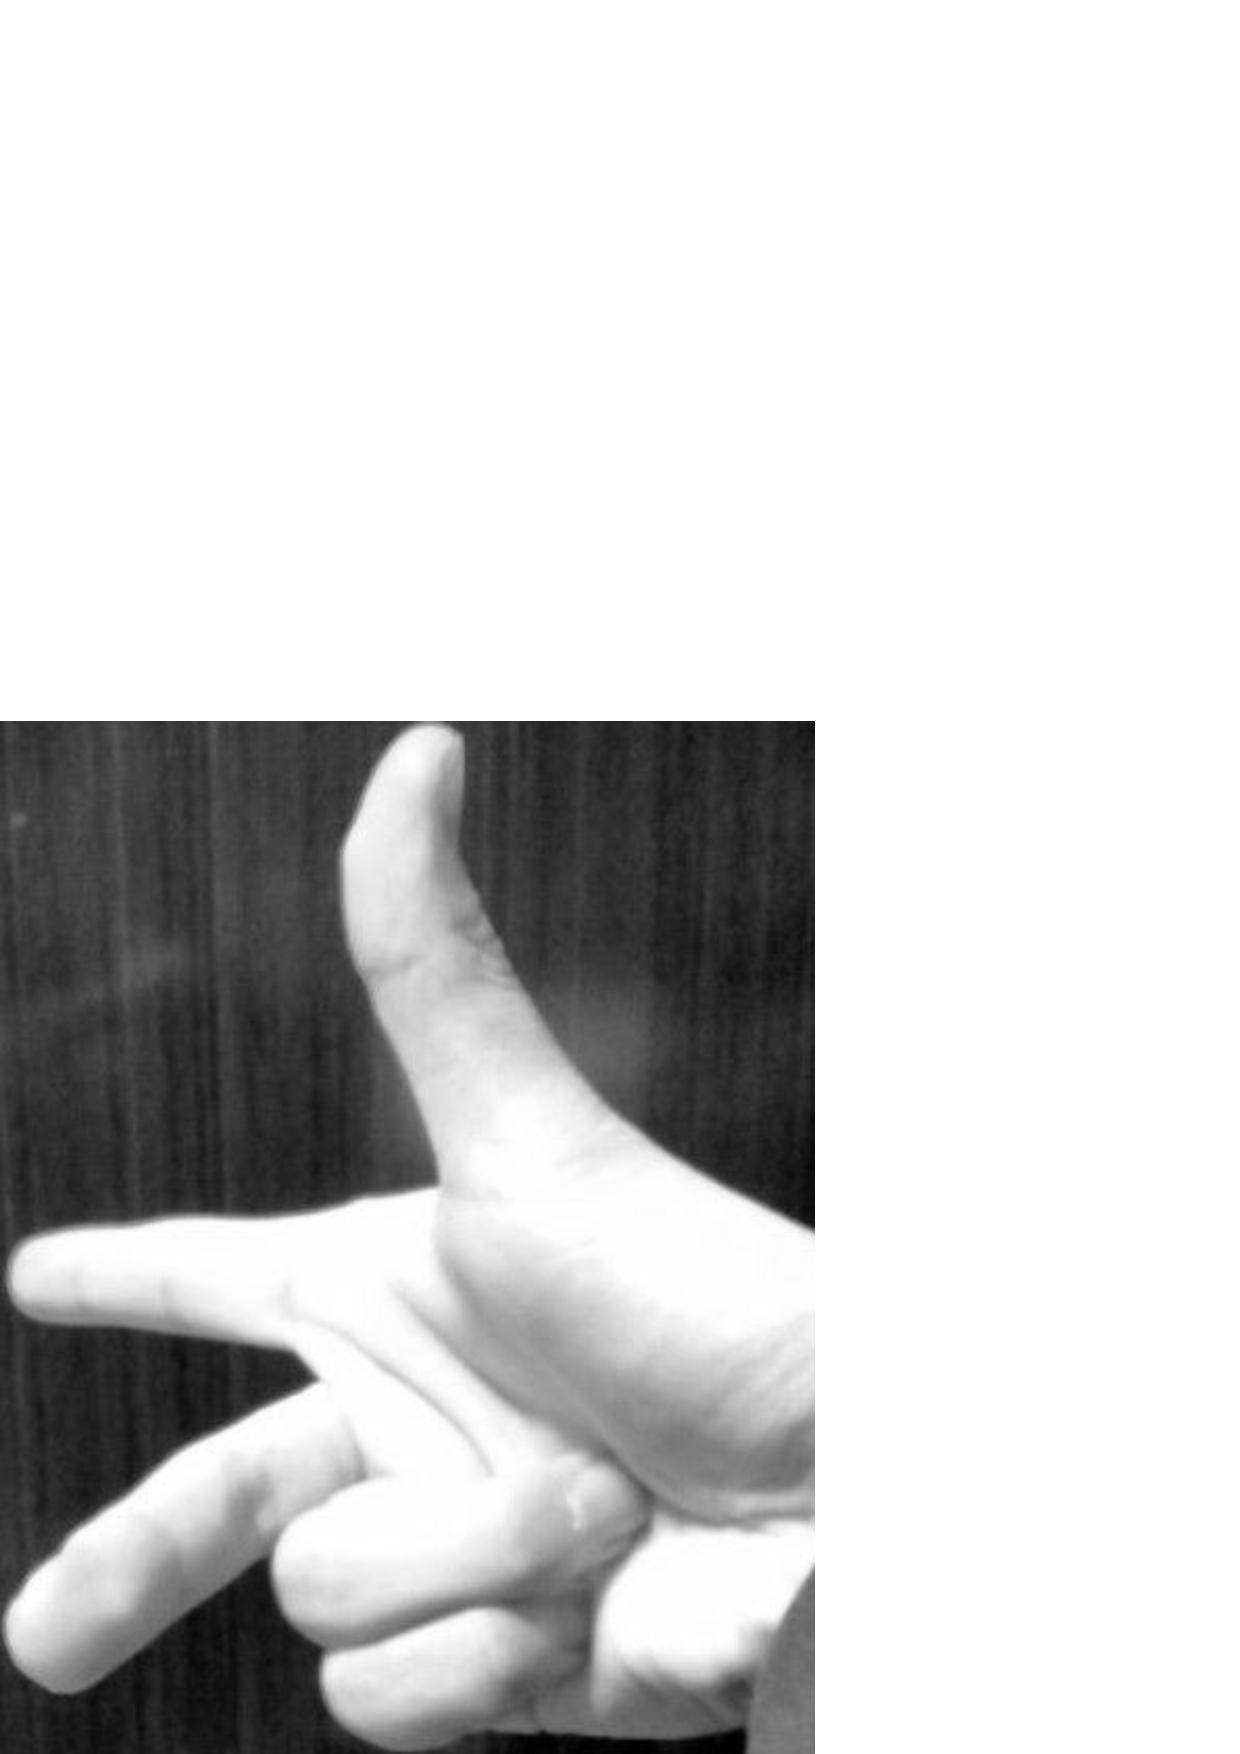
\includegraphics[keepaspectratio, width=3cm,height=3.75cm,clip]{migitekei_TE_2.pdf}

                                    (a) 右手
                                    \label{fig:migitekei_TE_mono_x}
                                \end{center}
                            \end{minipage}
                            \begin{minipage}{0.5\hsize}
                                \begin{center}
                                    \includegraphics[keepaspectratio, width=3cm,height=3.75cm,clip]{migineji_Myhand.pdf}

                                    (b) 対応図
                                    \label{fig:migineji_Myhand}
                                \end{center}
                            \end{minipage}
                        \end{tabular}
                        \caption{右手系}
                    \end{figure}
                \end{memo}

        \subsubsection{乗算?}
            ベクトルの乗算を,加算と同じように定義できないだろうか.
            つまり,2つの $n$ 次元ベクトル $\ba=(a_{1},\,a_{2},\,\cdots,\,n)$,
            $\bb=(b_{1},\,b_{2},\,\cdots,\,n)$ を用いて,
                \begin{equation*}
                    {(\ba \ast \bb)}_{i} = a_{i}b_{i}
                \end{equation*}
            と定義してはだめか
                \footnote{
                    記号に $\ast$ を使った理由は,内積の記号に $\cdot$,
                    外積の記号に $\times$ が使われるため,これらと区別
                    したかったためである.
                }.
            先人がこのように定義をしていないからには,
            できない理由があるに違いない.しかし,このように
            乗算を定義しても,不整合が起きるわけでもなく,定義不可能
            とは思えず,むしろ定義可能であると思えて仕方ない.
            私の力では,この定義を採用しない強い理由を見つけられない.

            しかし,このような乗算を定義してしまうと,ベクトルと数の違いが全く
            なくなってしまうことは確かだ
                \footnote{
                    実際に試してみてほしい.数と全く同じで,ベクトルを
                    定義した意味が全く感じられないことだろう.
                }.
            つまり,ベクトルとは表記上の利便性が向上
            しただけで,数学的な新しい概念となるわけではなくなる.
            数学的な発展を考えた場合,このような仕方の冗談の定義では
            前進がないので無駄ということになる.要するに,こんな乗算を定義
            してしまっては,わざわざベクトルを定義したことが無意味になって
            しまうのだ.表記方法を工夫しただけで新しい数学的概念とは言えない.
            もちろんこれでは,物理学にとっても,何のご利益もない
            ものになってしまうことだろう.
            だから,むしろ意識的に,このような定義を避けているのではない
            かと思われる(確証はない).ベクトルに内積や外積を定義することで,
            物理学に有用な数学になると共に,とても興味深い数学的対象となる.

        \subsubsection{除算??}
            ベクトルの内積の定義を採用すると,
            ベクトルの除算を定義することは難しい,と悟るのは容易だろう
            \footnote{
                $\bX\cdot\ba=k$ のとき,単純に $\ba=k/\bX$ とはできそうにない.
                $\bX$ をベクトルの変数とみなしたときに,この式を満たす $\bX$ は
                無限に存在するするから,できるとするならば,何か条件や約束事が必要だが,
                いい案は思い当たりそうにない.例えば,無限に存在する解をひとまとめにして,
                "解空間"(微分方程式など解空間とはべつもの)なるものをでっち上げたとしても,
                これ以上の発展は見込めないだろう.
            }.

            上記の "$\ast$" 乗算が採用されるのであれば,同じように除算を
            定義することは可能である.それは単に数を並べただけなので,
            吸うと全く同じ四則演算を定義すれば,不整合は起こらない.
            上記の乗算を定義しない理由に従うと,内積や外積を定義した方が
            学問的に有益である.そうなると,除算の定義が格段に難しくなる,
            というか,定義できたとしても条件が複雑すぎて,つまらなくなるだけだろう.

            だから,除算が定義できないのではなく,学問的に有益でないから定義しない
            と言ったほうが,正確なのであろう.

            数における0除算の禁止も,数学的に有益ではないから定義しないのだ,言えなくもない.
            よく挙げられる0除算が禁止される理由として,それを仮定すると不整合が起きるからだ
            といった説明がなされることがある
                \footnote{
                     $a$ を任意の数とするとき,$a \cdot 0 = 0$ が成立する(0の存在公理).
                     このとき,$a \neq b$ なる $b$ をもってきても $b \cdot 0 = 0$ である.
                     よって,$a \cdot 0 = b \cdot 0$(ここまでは正しい).
                     \textbf{両辺を0で割ると} $a=b$ となるが,これは $b$ の最初の条件に
                     矛盾する(不整合の発生).よって,0除算は禁止とされる.
                }.
            しかし,これは決して論理的な説明でない(美しい言い訳ではあるけれど).
            不整合が起きないように定義しなおせばよい.
            数学の論理は自然に存在するものではなく,人間が勝手気ままに構築
            するものであるから,定義なんていくらでも好き勝手できるはずである.ただ,
            0除算が定義できるようなうまい約束事を見つけられたとしても,複雑怪奇な理論
            が出来上がることになるのだろう(そんな理論に誰が興味を持つだろうか).

        \subsection{分解}
        1つのベクトルを複数のベクトルに分割することも可能である.
        例えば,$\ba = \bb + \bc$ が 成立しているとき,
        ベクトル $\ba$ は 2つのベクトル$\bb$と$\bc$に分割可能である.
        等式が成立していれば,分割するベクトルの個数に際限はない.
        このように,1つのベクトルを,加算が成り立つように複数のベクトルに
        分割することを,ベクトルの \textbf{分解} という.

        \subsection{単位ベクトル}
        大きさが1のベクトルを \textbf{単位ベクトル} という.
        単位ベクトルの記号は教科書により様々である.
        このノートでは,$\bn$ を単位ベクトルの記号として使用する
        \footnote{
            ただし,常にこの記号を用いるわけではない.その場合は,その直前か直後
            に説明を書くこととする.
        }.

        定義から,以下が成立する($n$ 次元を想定).
        \begin{align}
            |\bn| = \sqrt{\sum_{n=1}^{n} {n_{i}}^{2}} = 1.
        \end{align}
        $n_{i}$ のそれぞれの値には興味はないが,上記の関係式を満たす.
        単位ベクトルの方向は問わない.

                \subsection{演算の諸性質(公式)}
        \begin{mycomment}
            ベクトル基本的な演算性質を記しておく.
            $\ba$,$\bb$,$\bc$,$\bd$ はベクトルで,$k$,$l$ はスカラーである.
            括弧の内部の計算は,それがない部分よりも,優先度が高い(先に計算すべき)とし,
            それ以外の計算は左から順に計算する.
        \end{mycomment}

        \subsubsection{加算と定数倍に関する公式}
            ベクトルの加算と定数倍に関する演算性質は,スカラーの場合と変わらない.
            代表的な演算を以下に書いておく.
            \begin{enumerate}
                \item $\ba + \bb = \bb + \ba$
                \item $(\ba + \bb ) +\bc = \ba + (\bb + \bc)$
                \item $k (\ba + \bb) = k\ba + k\bb$
                \item $k(l\ba) = l(k\ba) =(kl)\ba$
                \item $\ba = \ba + \bzero = \bzero + \ba$
                \item $\ba +(-1)\ba = \bzero$
                \item $1\ba = \ba$
            \end{enumerate}

            以下,簡単に説明を与えておく.
            \begin{enumerate}
                \item 項の順序を入れ替えてから加算しても,結果は変わらない.\textbf{交換法則} とよばれる.
                \item 加算の順番を入れ替えても,結果は変わらない.\textbf{結合法則} とよばれる.
                \item 加算と定数倍に関する性質.
                      加算してから定数倍しても,両者を定数倍してから加算しても,どちらも
                      同じ結果になる.\textbf{分配法則} とよばれる.
                \item スカラーのかける順番を変えても,結果はわらなない.
                \item ゼロベクトル $\bzero$ を足しても結果は変わらない.
                      法則ではなく,$\bzero$ の存在を認めるもの.
                \item ベクトルから自身を引くとゼロベクトルになる.
                      $(-1)\ba$ は $\ba$ の \textbf{逆ベクトル} という.
                      $\ba$ も $(-1)\ba$ の逆ベクトルである(逆ベクトルの一意性).
                \item スカラーの1倍の1は記述を省略できる.
            \end{enumerate}

            どれも,定義から丁寧に計算すれば自明であるので,証明するまでもない
            \footnote{
                本音は$\cdots$
                \begin{itemize}
                    \item "記述が面倒だから省略させてほしい" という甘え
                    \item "書いたところで,ノートの記述が煩雑になって読みにくくなる" という言い訳
                    \item "自分で計算すれば,理解の確認になるのではないか" という逃げ
                \end{itemize}
                である.

                証明するには,式の両辺を独立に成分計算し,
                対応する成分同士が等しいことを確認すればいい.
                一意性を示したい場合には,異なる2つのものがあると仮定しても,
                両者が同値になることを示せばいい.
            }.

        \subsubsection{内積に関する公式}
            内積もスカラーと同じように扱える.主な性質は以下の通り.
            \begin{enumerate}
                \item $\ba \cdot \ba = {|\ba|}^{2}$
                \item $\ba \cdot \bb = \bb \cdot \ba$
                \item $\ba \cdot (\bb + \bc) = \ba \cdot \bb + \ba \cdot \bc$
                \item $(\ba + \bb) \cdot \bc = \ba \cdot \bc + \bb \cdot \bc$
                \item $k(\ba \cdot \bb) = (k\ba) \cdot \bb = \ba \cdot (k\bb)$
                \item $\ba \parallel \bb \Leftrightarrow \ba \cdot \bb = 0$
                \item $\ba \perp \bb \Leftrightarrow \ba \cdot \bb = \displaystyle\frac{\pi}{2}$
            \end{enumerate}

            言葉でも説明しておこう.
            \begin{enumerate}
                \item 自身の内積は,自身の大きさの2乗に等しい.
                \item 内積の項の順序を入れ替えても,結果は変わらない.
                \item 分配法則が成り立つ
                \item 分配法則の別の形(1と2より自明だろう)
                \item 定数倍と内積に関して,結合法則が成り立つ.
                \item 2つのベクトルが平行であることと,それらの内積が0であることは等価
                \item 2つのベクトルが垂直であることと,それらの内積が$\displaystyle\frac{\pi}{2}$であることは等価
            \end{enumerate}

            \begin{mysmallsec}{内積の使い所}
                物理学でベクトルの内積を使う場合は,2つのベクトルの交わりの角度を気にする場合が
                ほとんどである.平行なのか,垂直なのか,そうでなければどんな角度で交わっているのかが,
                内積の計算によってわかるからである.
            \end{mysmallsec}

        \subsubsection{外積に関する公式}
            外積の演算性質は,他とは異なるので,注意が必要である.
            \begin{enumerate}
                \item $\ba \times \ba = \bzero$
                \item $\ba \times \bb = - \bb \times \ba$
                \item $\ba \times (\bb \times \bc) = (\ba \cdot \bc) \bb - (\ba \cdot \bb) \bc $
            \end{enumerate}

            簡単にコメントを書いておく.
            \begin{enumerate}
                \item 自身の外積はゼロベクトルである.
                \item 外積の項の順序入れ替えると,符号が反転する.
                \item \textbf{ベクトルの三重積} という異名をもつ.
                      ちなみに,右辺の $\ba \cdot \bc$,$\ba \cdot \bb$ の演算結果はスカラーである.
            \end{enumerate}

            他にもたくさんあるけど,省略する.ベクトルの外積に関する公式は,
            一見して複雑な形をしたものが多く(検算が大変),挫折しがちだ.
            しばらく見ていると規則性が見えてきて,美しく感じるのかもしれないが,
            頻繁に使うのは上の3つくらいだ.後は,必要になったらときに,公式集を参照しよう.

        \subsubsection{単位ベクトルに関する公式}
        任意のベクトルは,同じ向きの単位ベクトルの定数倍である
            \footnote{
                証明はしないけど.
            }.
        アタリマエのことを言っているようだが,確認しておこう.
        ある $n$ 次元ベクトルを用意して,$\bX$ としよう.
        単位ベクトルの向きは,$\bX$ と同じとする.
        $\bX$ を単位ベクトル $\bn$ の定数 $k$ 倍と表せたとすると,$\bX = k\bn$ と
        なる.$\bX=(X_{1},\,X_{2},\,\cdots)$,$\bn=(n_{1},\,n_{2},\,\cdots,\,n)$ とすると,
            \begin{equation*}
                X_{i} = kn_{i} \quad,\quad (i=1,\,2,\,\cdots,\,n)
            \end{equation*}
        が成り立つ.これを踏まえて,$\bX$ の大きさ $|\bX|$を考えてみよう.
        簡単な計算で,$|\bX|=k$ が導ける.
            \begin{equation*}
                |\bX| = \sqrt{\sum_{n=1}^{n} {X_{i}}^{2}}
                      = \sqrt{\sum_{n=1}^{n} {(kn_{i})}^{2}}
                      = k \left(\sqrt{\sum_{n=1}^{n} {n_{i}}^{2}}\,\right)
                      = k \cdot 1
                      = k.
            \end{equation*}
        ここで,単位ベクトルの大きさが1であることを使用した.

        以上から,任意のベクトルは単位ベクトルを自身の大きさで定数倍したものに等しい,と言える.
        式で書くと,次の通り.
        \begin{align}
            \bX = |\bX|\bn.
        \end{align}

        上式を逆手に考えて,
        \begin{align}
            \bn = \frac{\bX}{|\bX|}= \frac{1}{|\bX|} \bX.
        \end{align}
        と見ることで,任意のベクトルの単位ベクトルを計算することもできる.

        しかし,次は無意味であることに注意しておくこと.
        \begin{align*}
            \mbox{(意味のない式)}\quad|\bX| = \frac{\bX}{\bn}
        \end{align*}
        ベクトル同士の除算は定義されておらず,この式は何も意味しない.

